\documentclass{beamer}
\usetheme{Madrid}
\usepackage[italian]{babel}

\title[Trading AI]{Progettazione e sviluppo di test suite automatica e modulo raccolta dati per intelligenze artificiali che si occupano di creare strategie di investimento}
\author{Garion Musetta}
\centering
\date{Aprile 2020}
\begin{document}
\maketitle

\begin{frame}{Contesto}
\begin{itemize}
\item Nexid Edge blockchain e AI sviluppa strumenti intelligenti per l’analisi del mercato delle criptovalute e
la creazione di strategie di investimento.\\ Inoltre realizza Smart Contract sulla Blockchain Ethereum per la certificazione di opere in diversi tipi di settori.
\item Ha creato una AI in grado di prevedere il mercato finanziario delle criptovalute e di creare \textbf{strategie di investimento} intelligenti (Sentyment AI).
\end{itemize}
\begin{figure}
    \subfigure{
\includegraphics[width=.2\linewidth]{nexid}}
    \subfigure{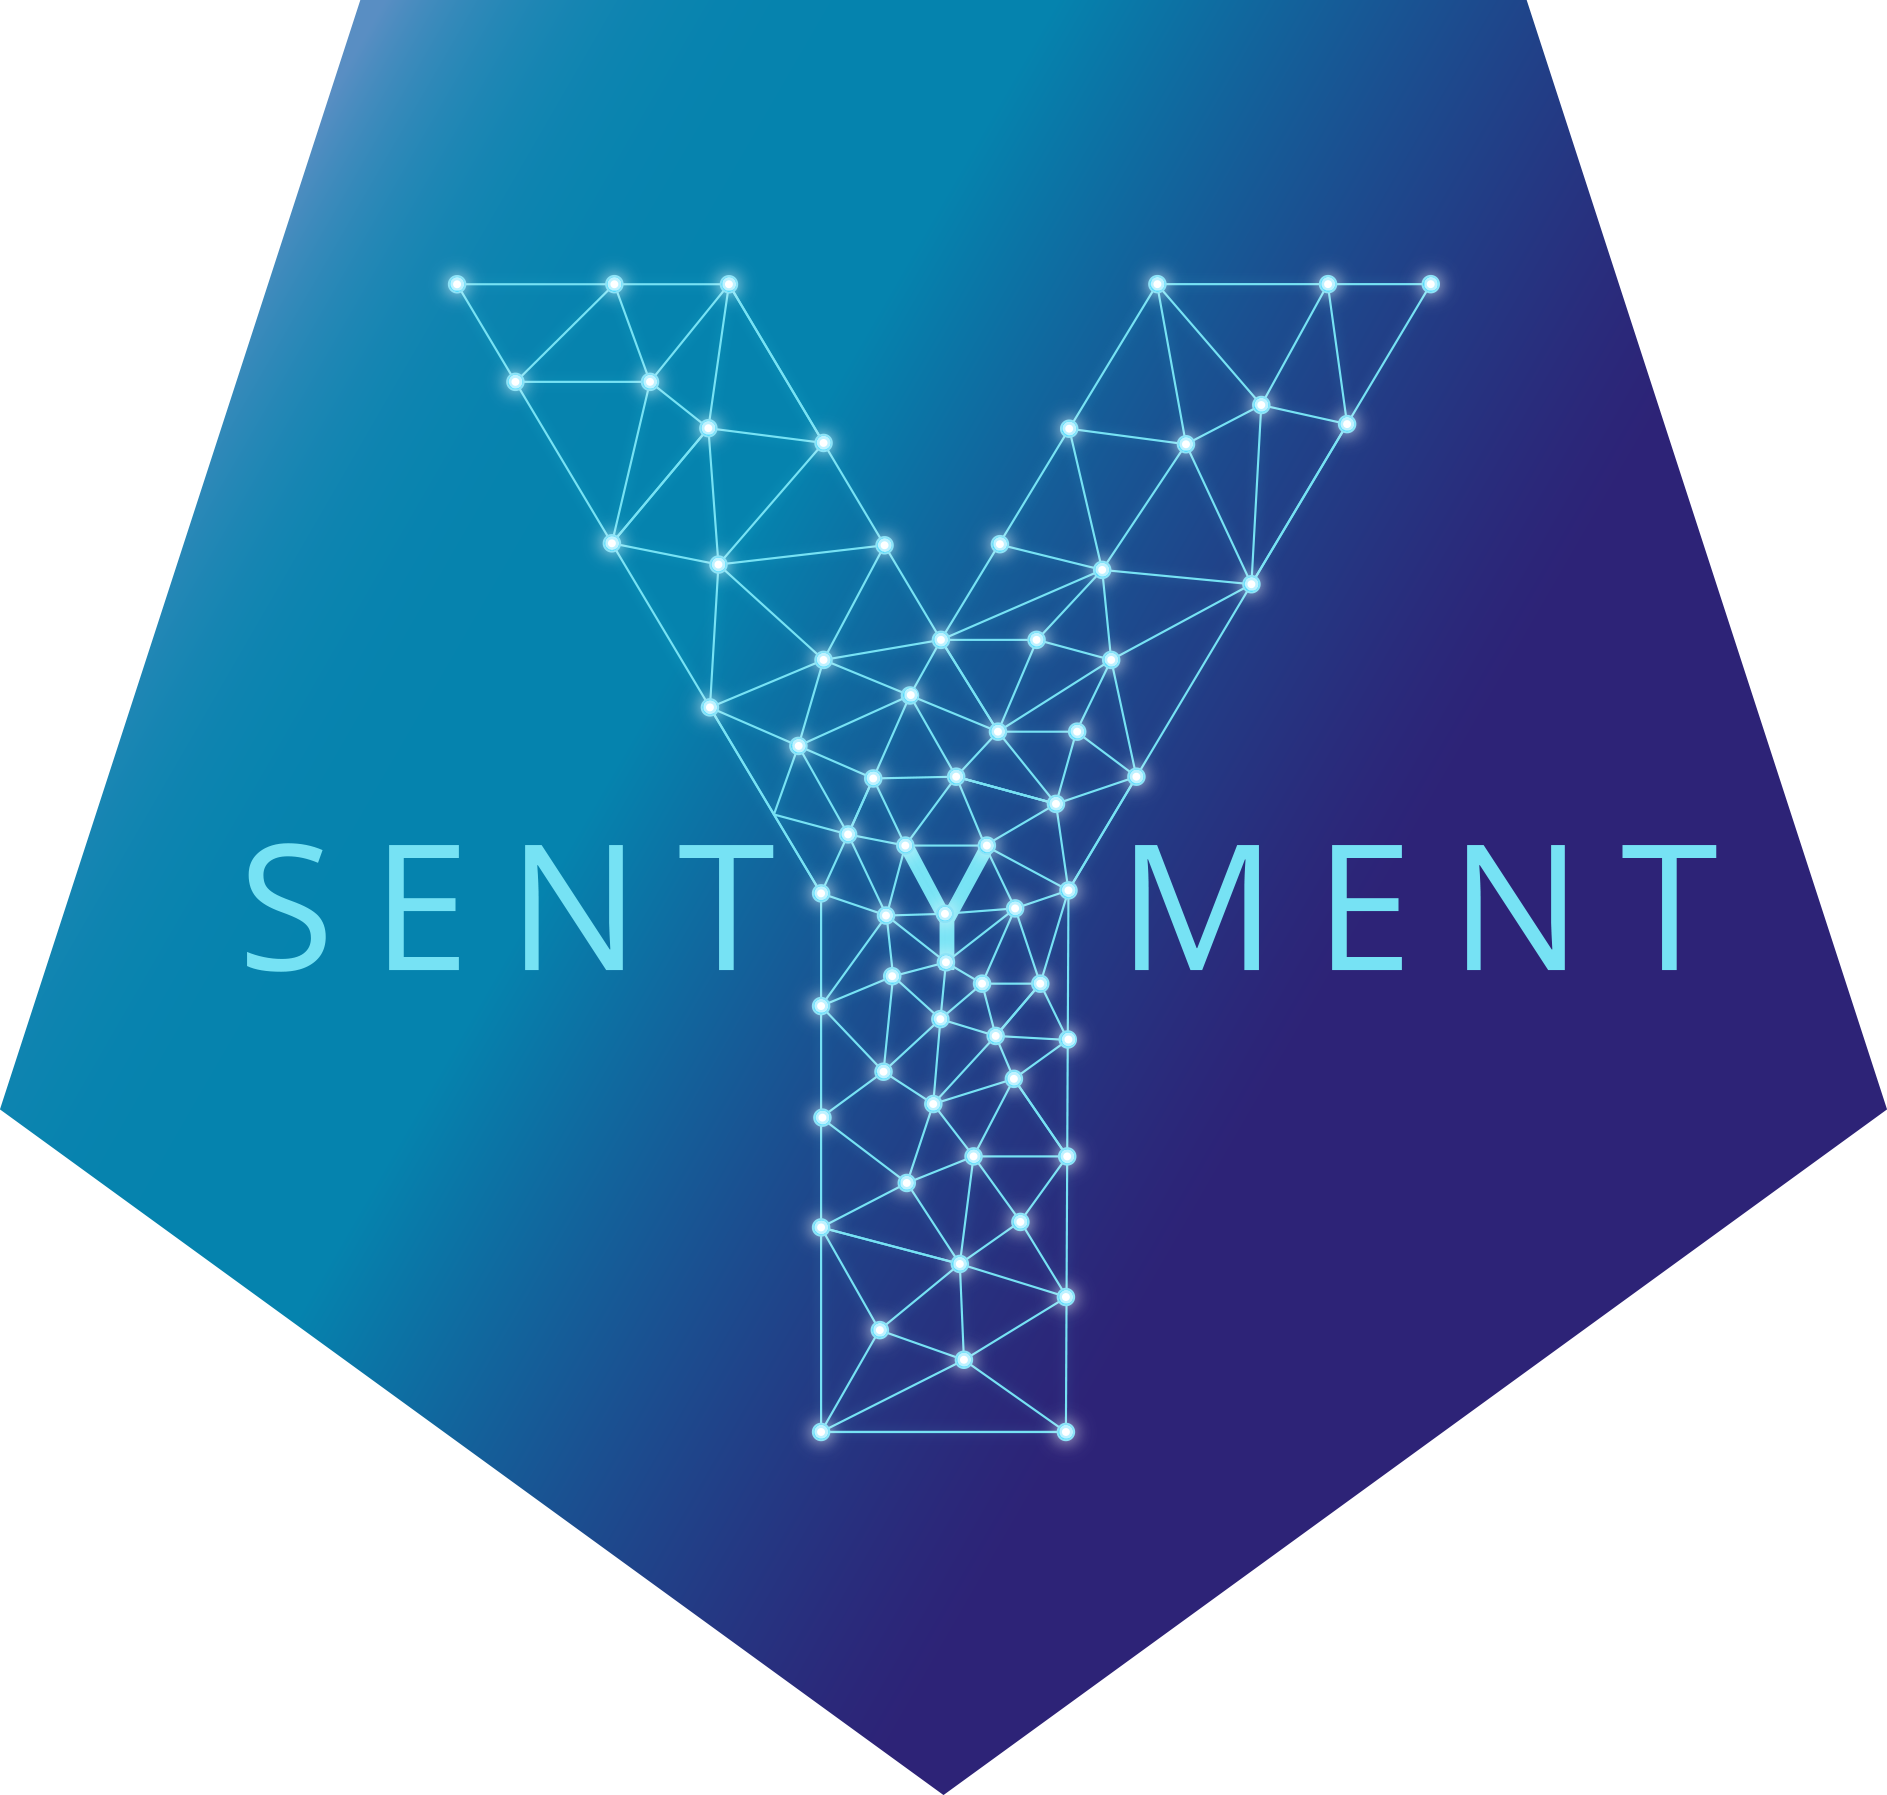
\includegraphics[width=.2\linewidth]{sentyment_logo}}
\end{figure}
\end{frame}

\begin{frame}{Previsione di mercato e serie temporali}
\begin{itemize}
\item In letteratura molti strumenti di AI raggiungono precisioni notevoli, con precisione sulla predizione dei valori fino a 80\%
\item Principalmente usano \textit{Neural Network}, \textit{Case Based Reasoning} e \textit{Support Vector Machine}. I metodi statistici sono ormai stati superati
\item Esiste molta varietà di approcci e i risultati migliori sono dati da combinazioni di tecniche: CBR+fuzzy/Genetic, NN+fuzzy/Genetic. Ggenetic usato per scelta topologia rete
\item Necessaria anche integrazione delle notizie di giornale su eventi quotidiani: text mining
\end{itemize}
\end{frame}

\begin{frame}{Previsione di mercato e serie temporali}
\begin{itemize}
\item Non è tuttavia dimostrato se il mercato sia predicibile o no (\textit{Efficient Market Hypothesis}).
Servirebbero dei lavori inconfutabili che non esistono ancora.
\item Lo strumento di Nexid non effettua previsioni puntuali di prezzi, ma diversifica il portfolio e sceglie in modo intelligente varie strategie di investimento in base all'andamento del mercato.
\item Sentyment AI opera su diverse criptovalute:
\begin{itemize}
    \item Ogni criptovaluta ha associato un insieme di AI separate e ognuna effettua predizioni crea strategie. \item Sono tutte simili fra loro ma hanno parametri differenti e agiscono in modo leggermente diverso.
    \item Per ogni valuta, solo la migliore è usata
\end{itemize}
\end{itemize}
\end{frame}

\begin{frame}{Financial Trading}
\begin{itemize}
    \item Acquistando (\textit{buy}) un asset per un certo prezzo e rivendendolo (\textit{sell}) quando il valore è salito si ottiene un guadagno
    \item Ripetendo l'operazione con il budget appena ricavato, per investirlo nuovamente, è possibile generare ricchezza. 
    \item Una strategia di investimento fa uso di uno o più indicatori statistici per definire i punti in cui comprare o vendere un titolo.
    \item Analizzando l'andamento di un mercato è possibile farsi un'idea di come evolve e scegliere una strategia opportuna.
    \begin{figure}
    \subfigure{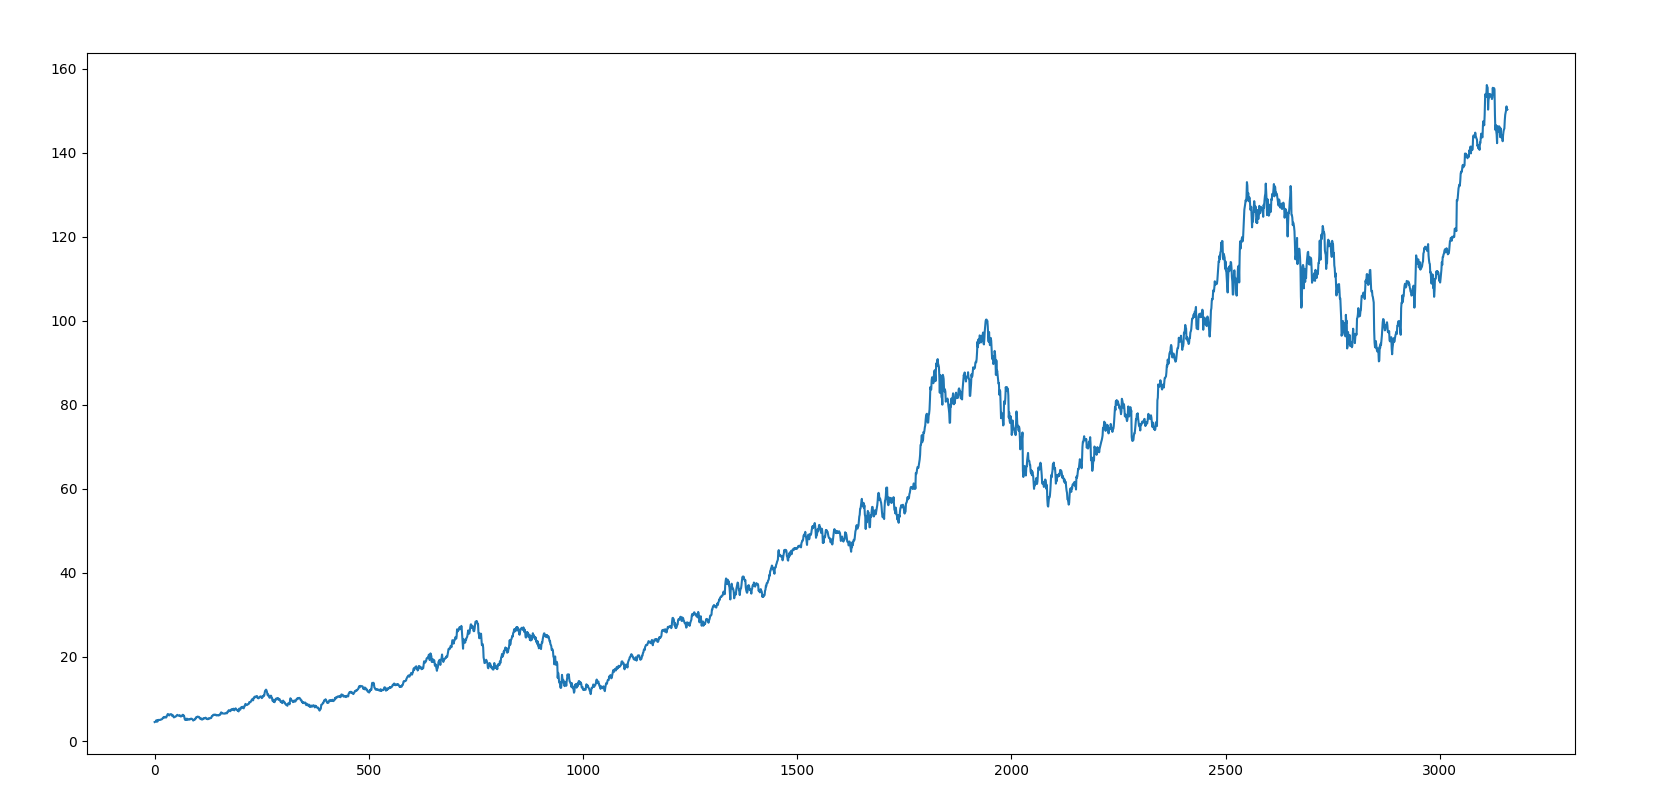
\includegraphics[width=.3\linewidth]{stock1}}
    \subfigure{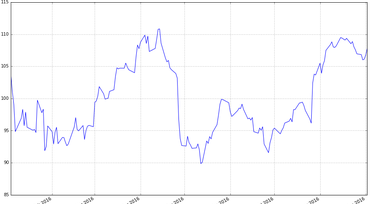
\includegraphics[width=.3\linewidth]{stock2}}
    \subfigure{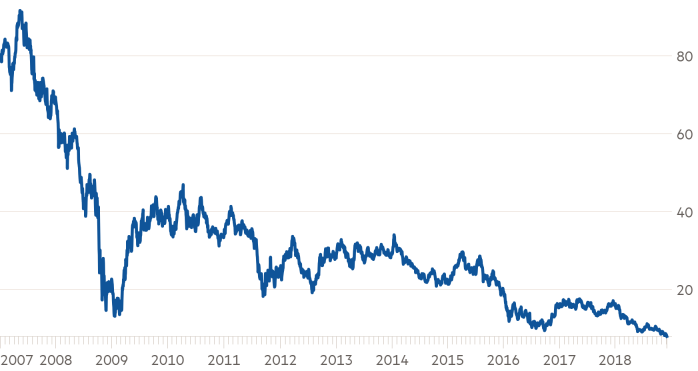
\includegraphics[width=.3\linewidth]{stock3}}
\end{figure}
\end{itemize}
\end{frame}

\begin{frame}{Strategie di investimento}
\begin{itemize}
    \item Generalmente si cerca di comprare quando il titolo ha prezzo basso e vendere quando è alto: \textit{buy} nelle valli e \textit{sell} nei picchi. 
    \item L'operazione va effettuata sul breve periodo (su base giornaliera / settimanale) e ripetuta spesso
    \item È difficile prevedere il preciso andamento e quindi si usano indicatori che lo riassumono
    \item Se si analizza che il mercato è in forte crescita senza eccessive perdite si può optare per BUY-HOLD: compra all'inizio e mantiene il titolo fino alla fine.
    \item Se però il mercato dovesse crollare, buy hold segue di conseguenza
\end{itemize}
\end{frame}

\begin{frame}{Strategie di investimento}
\framesubtitle{Strategie più complesse per il breve termine}
\begin{itemize}
    \begin{block}{SMA}
    Simple Moving Average. Strategia che segnala i cambi di tendenza grazie a due medie mobili, una breve (5 / 10 giorni) e una lenta (100 / 200). Le linee delle medie sono tracciate sul grafico dei prezzi e, quando avviene un'intersezione fra le due, si genera un segnale di \textit{buy} o \textit{sell}.\\ Quando la media breve supera quella lenta il segnale è \textit{buy}. Se la media lenta supera quella veloce si ha la situazione opposta e un segnale di \textit{sell}
    \end{block}
    \begin{figure}
        \centering
        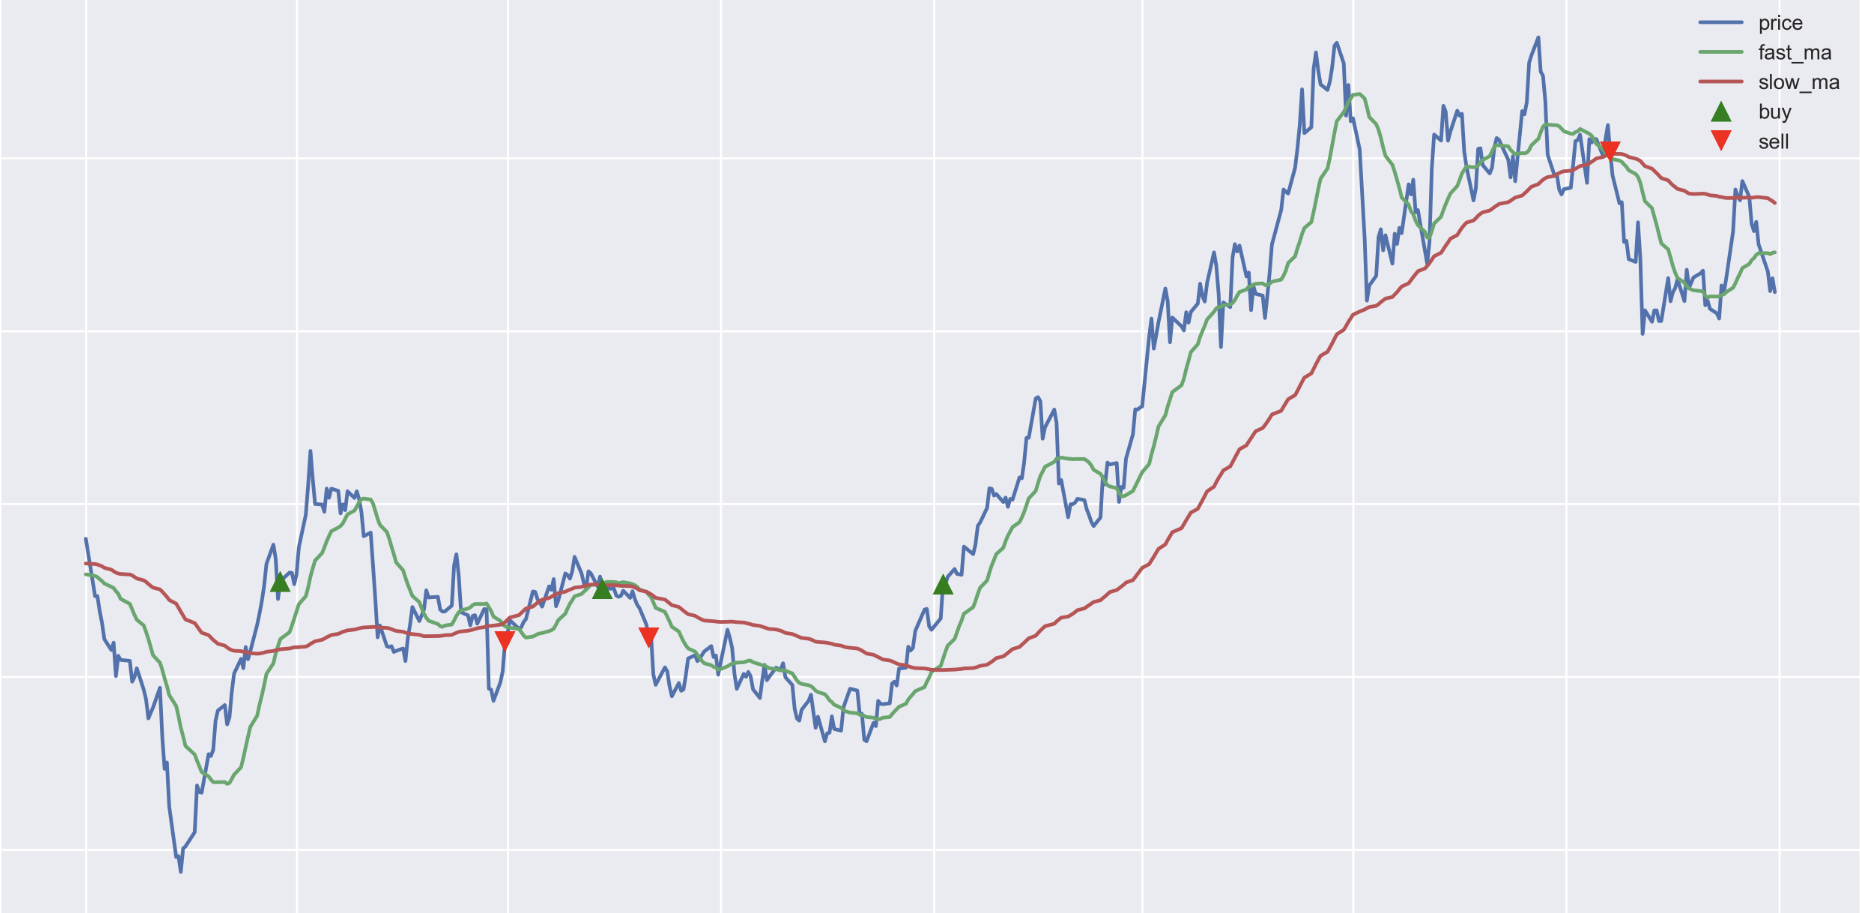
\includegraphics[width=.5\linewidth]{moving_avg2}
    \end{figure}
\end{itemize}
\end{frame}

\begin{frame}{Scopo della tesi}
\begin{itemize}
\item Sentyment AI sceglie in modo intelligente quale strategia applicare a seconda delle varie situazioni,
dell'andamento dei prezzi e del valore degli indcatori.
\item Sentyment AI opera su diverse criptovalute. Ogni criptovaluta ha associato un insieme di AI separate
\item L'obiettivo è sviluppare uno strumento in grado di stabilire, a intervalli di tempo da definire,
quale sia la AI migliore all'interno di ciascun insieme: \textit{meta-learner}
\item Stabilita la migliore, la si può etichettare come "attiva" ed usare in produzione, permettendogli di piazzare direttamente ordini di acquisto e vendita sul mercato.
\end{itemize}
\end{frame}

\begin{frame}{Scelta della migliore AI: \textit{meta-learner}}
\begin{itemize}
\item
\end{itemize}
\end{frame}



\begin{frame}{Content}
\begin{itemize}
\item What is machine learning? 
\item Growth of Machine Learning.
\item Application of machine Learning. 
\item Classification:  Applications
 \item Top 10 use cases of Machine Learning
 \item What machine learning tools do Kaggle champions use?
    \item Types of Learning? 
\end{itemize}
\end{frame}
\begin{frame}{What is Machine learning?}
\framesubtitle{Why do we need to care about machine learning?}
\begin{itemize}
    \item Machine learning (ML) is a category of algorithm that allows software applications to become more accurate in predicting outcomes without being explicitly programmed. The basic premise of machine learning is to build algorithms that can receive input data and use statistical analysis to predict an output while updating outputs as new data becomes available.
    \item Writing software is the bottleneck, we don’t have enough good developers. Let the data do the work instead of people. Machine learning is the way to make programming scalable.
    \item Machine Learning is getting computers to program themselves. If programming is automation, then machine learning is automating the process of automation.
\end{itemize}
\end{frame}
\begin{frame}{Growth of Machine Learning}
   \begin{itemize}
       \item Machine learning is preferred approach to
       \item Speech recognition, Natural language processing
       \item Computer vision
       \item Medical outcomes analysis
    \item Robot control
    \item Computational biology
    \item Improved machine learning algorithms
    \item Improved data capture, networking, faster computers
    \item Software too complex to write by hand
    \item New sensors / IO devices
\end{itemize}
\end{frame}

\begin{frame}{Applications of Machine Learning}
  \framesubtitle{Sample applications of machine learning:}
  The value of machine learning technology has been recognized by companies across several industries that deal with huge volumes of data. By leveraging insights obtained from this data, companies are able work in an efficient manner to control costs as well as get an edge over their competitors. This is how some sectors / domains are implementing machine learning -
  \begin{itemize}
      \item Financial Services
      \item Marketing and Sales
      \item Government
      \item Healthcare
      \item Transportation
      \item Oil and Gas
  \end{itemize}
 
\end{frame}
\begin{frame}
\frametitle{Sample application of Machine Learning}
 
\begin{block}{Financial Services}
Companies in the financial sector are able to identify key insights in financial data as well as prevent any occurrences of financial fraud, with the help of machine learning technology. The technology is also used to identify opportunities for investments and trade. Usage of cyber surveillance helps in identifying those individuals or institutions which are prone to financial risk, and take necessary actions in time to prevent fraud.
\end{block}
 
\begin{block}{Marketing and Sales}
Companies are using machine learning technology to analyze the purchase history of their customers and make personalized product recommendations for their next purchase. This ability to capture, analyze, and use customer data to provide a personalized shopping experience is the future of sales and marketing.
\end{block}
\end{frame}
\begin{frame}
\begin{block}{Government}
Government agencies like utilities and public safety have a specific need FOR Ml, as they have multiple data sources, which can be mined for identifying useful patterns and insights. For example sensor data can be analyzed to identify ways to minimize costs and increase efficiency. Furthermore, ML can also be used to minimize identity thefts and detect fraud.
\end{block}
\begin{block}{Healthcare}
With the advent of wearable sensors and devices that use data to access health of a patient in real time, ML is becoming a fast-growing trend in healthcare. Sensors in wearable provide real-time patient information, such as overall health condition, heartbeat, blood pressure and other vital parameters. Doctors and medical experts can use this information to analyze the health condition of an individual, draw a pattern from the patient history, and predict the occurrence of any ailments in the future. The technology also empowers medical experts to analyze data to identify trends that facilitate better diagnoses and treatment.
\end{block}
\end{frame}
\begin{frame}
    \begin{block}{Transportation}
    Based on the travel history and pattern of traveling across various routes, machine learning can help transportation companies predict potential problems that could arise on certain routes, and accordingly advise their customers to opt for a different route. Transportation firms and delivery organizations are increasingly using machine learning technology to carry out data analysis and data modeling to make informed decisions and help their customers make smart decisions when they travel.
    \end{block}
    \begin{block}{Oil and Gas}
    This is perhaps the industry that needs the application of machine learning the most. Right from analyzing underground minerals and finding new energy sources to streaming oil distribution, ML applications for this industry are vast and are still expanding.
    \end{block}
\end{frame}

\begin{frame}{Classification: Applications}
    \begin{itemize}
        \item Aka Pattern recognition
\item Face recognition: Pose, lighting, occlusion (glasses, beard), make-up, hair style 
\item Character recognition: Different handwriting styles.
\item Speech recognition: Temporal dependency. 
\item Use of a dictionary or the syntax of the language. 
\item Sensor fusion: Combine multiple modalities; eg, visual (lip image) and acoustic for speech
\item Medical diagnosis: From symptoms to illnesses
\item Web Advertizing: Predict if a user clicks on an ad on the Internet.
\end{itemize}
\end{frame}

\begin{frame}{Main Application}
    \begin{itemize}
        \item Face Recognition
        \item Prediction: Regression
        \item Regression Applications
    \end{itemize}
\end{frame}

\begin{frame}{Top 10 use cases of Machine Learning}
\includegraphics[height=6.8cm]{1_kTnSJQpzGw_w4uQKa_j7VQ.png}
\centering
\end{frame}

\begin{frame}{What machine learning tools do Kaggle champions use?}
 \includegraphics[height=6.8cm]{D3Pb_Q3UIAAuSWU.jpg}
\centering   
\end{frame}

\begin{frame}{Types of Learning?}
\begin{itemize}
    \item Supervised Learning: Uses
    \item Unsupervised Learning
    \item Reinforcement Learning
\end{itemize}
\end{frame}

\begin{frame}{Supervised Learning: Uses}
   \begin{block}{Prediction of future cases}
   Use the rule to predict the output for future inputs
   \end{block}
   \begin{block}{Knowledge extraction}
 The rule is easy to understand
   \end{block}
   \begin{block}{Compression}
  The rule is simpler than the data it explains
   \end{block}
   \begin{block}{Outlier detection}
   Exceptions that are not covered by the rule, e.g., fraud
   \end{block}
  
\end{frame}

\begin{frame}{Unsupervised Learning}
    \begin{itemize}
        \item Learning “what normally happens”
\item No output
\item Clustering: Grouping similar instances
\item Other applications: Summarization, Association Analysis. \end{itemize}
\begin{block}{Example applications}
\begin{itemize}
    \item Customer segmentation in CRM
\item Image compression: Color quantization
\item Bioinformatics: Learning motifs
\end{itemize}
\end{block}
\end{frame}

\begin{frame}{Reinforcement Learning}
    \begin{itemize}
        \item No supervised output but delayed reward
        \item Policies: what actions should an agent take in a particular situation.Utility estimation: how good is a state (used by policy)
        \item Credit assignment problem (what was responsible for the outcome) 
     \end{itemize}
     \begin{block}{Applications}
     \begin{itemize}
        \item Game playing
        \item Robot in a maze
        \item Multiple agents, partial observability, ...
     \end{itemize}
     \end{block}
   \end{frame}

\begin{frame}
\huge{\centerline{The End}}
\end{frame}

\end{document}
